\TODO[]{Finish Results }
\TODOMaybe{Flesh out more sub-sections}

\draftText{%
  Parse initial study. \\
  Get a feeling for the personas -> observe workflows. \\

  < Manager / Lead >
  \begin{itemize}
    \item{Better overviews}
    \item{Task creation + dispatch}
    \item{Easier input, fewer fields}
    \item{Kanban board for users}
  \end{itemize}

  < Artist >
  \begin{itemize}
    \item{Automation of communication back to manager/lead}
    \item{More collaborative information, "anyone else also working on this?"}
    \item{Auto-completion of information}
    \item{More rigid and centralized info-repository (ex. permanent chat log on
      discussion of specific ticket.)}
    \item{Force information that obscures the process if missing, ex, why is
        this blocked?}
    \item{Easier handling of media uploads, screenshots etc.}
  \end{itemize}

  < Animator >
  \begin{itemize}
    \item{Automatic cascading of skipped tasks -> skip child-tasks}
    \item{Filter or compress similar information}
    \item{Information in flux}
  \end{itemize}

  < System-Architect / Maintainer / Coordinator >
  \begin{itemize}
    \item{Better integration with current tooling}
    \item{Better formatted gantt-chart}
    \item{Batch creation of tasks}
  \end{itemize}
}
{
  \begin{figure}[H]
    \centering
    \begin{subfigure}[b]{0.475\textwidth}
      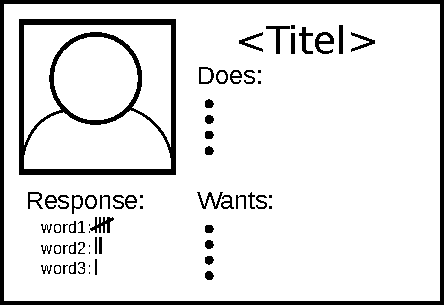
\includegraphics[width=\textwidth]{images/template_persona.pdf}
      \caption{Persona description \#1}
    \end{subfigure}
    \hfill
    \begin{subfigure}[b]{0.475\textwidth}
      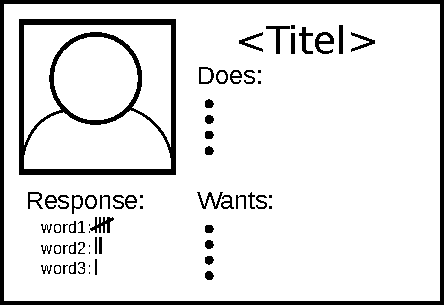
\includegraphics[width=\textwidth]{images/template_persona.pdf}
      \caption{Persona description \#2}
    \end{subfigure}

    \vskip\baselineskip

    \begin{subfigure}[b]{0.475\textwidth}
      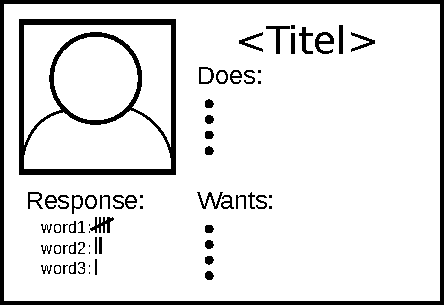
\includegraphics[width=\textwidth]{images/template_persona.pdf}
      \caption{Persona description \#3}
    \end{subfigure}
    \hfill
    \begin{subfigure}[b]{0.475\textwidth}
      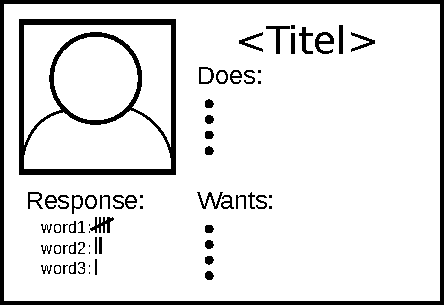
\includegraphics[width=\textwidth]{images/template_persona.pdf}
      \caption{Persona description \#4}
    \end{subfigure}
    \caption{Persona descirptions.}
  \end{figure}
  This is the resulting text.
}
